\documentclass[conference]{IEEEtran}
% packages
\usepackage[T1]{fontenc}
\usepackage{cite}
\usepackage{url}
\usepackage[hidelinks,hypertexnames=false]{hyperref}
\usepackage{comment}
\usepackage{float}
\usepackage{graphicx}
\usepackage{amsmath,amssymb}
\usepackage{booktabs}
\usepackage{array}
\usepackage{comment}
\usepackage{listings}
\usepackage{algorithm}
\usepackage{algpseudocode}
\usepackage{xspace}
\graphicspath{{figures/}{paper/figures/}}

% custom commands
\newcommand{\privoke}{\textsc{PriVoke}\xspace}

% default setting overrides
\IEEEoverridecommandlockouts

%
\begin{document}
\title{\privoke: Supporting Detail}
\author{\IEEEauthorblockN{Nicholas Bisset, Manpreet Sahadevan, Nixon Ngai, and Sanoop Mallissery}}
\maketitle
\raggedbottom
\renewcommand{\thefigure}{S\arabic{figure}}
\renewcommand{\thetable}{S\Roman{table}}
\renewcommand{\theequation}{S\arabic{equation}}
This companion preserves detailed protocols, supporting outcomes and diagrams for \href{main.pdf}{the main paper}. It provides additional evidence and does not replace the main paper's methods, principal findings or limitations. It makes no assumption about whether supplementary material is accepted under the assessment rules.

\section*{Detailed System Diagrams}
Figures~\ref{fig:enforcement} and~\ref{fig:updates} expand the request and revision paths summarized in the main paper. Their captions retain the conditions that distinguish a request action from content transformation and a completed fit from an accepted publication.

\begin{figure}[t]
\centering
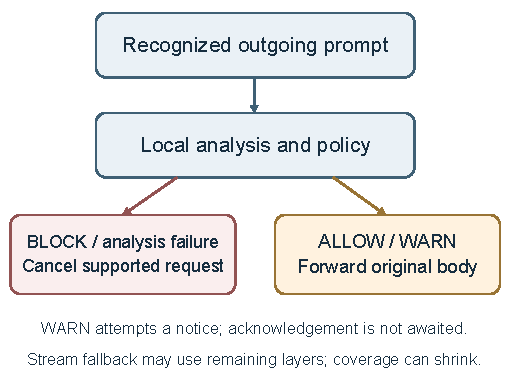
\includegraphics[width=\columnwidth]{architecture-enforcement.pdf}
\caption{Pre-transmission enforcement on supported hooks. WARN forwards unchanged content after attempting a notice; it does not wait for user acknowledgement. Analysis failure and reduced-layer stream fallback are distinct conditions. Disabled protection and unsupported traffic lie outside this decision path.}
\label{fig:enforcement}
\end{figure}

\begin{figure}[t]
\centering
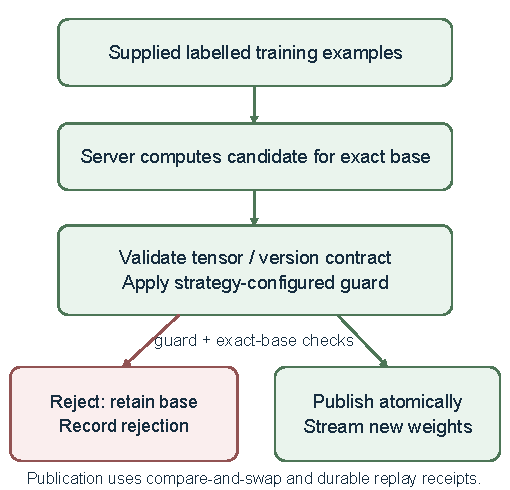
\includegraphics[width=\columnwidth]{architecture-updates.pdf}
\caption{A candidate is evaluated before publication. Compare-and-swap rejects stale/conflicting bases; durable receipts prevent an identical retry from applying twice. A passing retention guard covers its declared cases and criteria only. Head and underlying-model stages are separate publications, so a later rejection need not undo an earlier accepted head stage.}
\label{fig:updates}
\end{figure}

\appendices


\section{Exact Policy Representation}
\label{app:policy}
The representation separates what information a prompt contains from the context in which it is disclosed. Sensitivity S0--S3 denotes, respectively, no identified risk, low-risk personal context, potentially harmful personal information, and highly sensitive/identifying details or secrets. Audience, called visibility in the implementation, uses P0--P4/PU for public, semi-public, authentication-restricted, group-private, personal-private and unspecified context. The category set can contain more than one of ten labels: HEALTH, POLITICS, RELIGION, CRIMINAL, FINANCIAL, SEXUAL, CHILD, LOCATION, IDENTITY and THIRD\_PARTY.

The deterministic policy normally maps S3 to BLOCK and S2 to WARN. S0/S1 remain ALLOW unless IDENTITY and LOCATION coexist or either appears with P2--P4 visibility. A returned confidence below 0.5 moderates S3 to WARN and S2 without IDENTITY/LOCATION to ALLOW; other low-confidence classifications also become ALLOW. Aggregation preserves individual enforcement decisions, unions categories and retains the strongest sensitivity and known visibility. This specifies how the software derives an action, while leaving disclosure authorization and probability calibration as separate validation questions.

\section{Detailed Comparison Protocols and Terminology}
\label{app:protocols}
Repository protocol names identify the recipes and execution scopes behind the main-text comparisons. V1 denotes historical packages and AU3-selected V3 the updated packages. PH3 fits task heads over frozen encoders, EN3 continues encoder and head training together, and AU3 adds audience-supervised rehearsal. PIPE3 is the full-product comparison; HEADS/FULL contrasts head-only and full-model continuation. Reusing a protocol's result elsewhere in the paper does not create an additional independent study.
\subsection{Training Lineage and Selection}
Before assessment, the historical online studies specified artifacts, curricula, trainable tensors, seeds, budgets and safety/retention predicates. Their records keep accepted and rejected attempts separate, preventing an attempted update from being counted as a successful publication. Later semantic-only HEADS/FULL and representation studies likewise recorded explicit execution scopes and distinguished qualification from publication. Complete specifications and unsuccessful attempts remain in the repository research records alongside the reported outcomes.

The final packages descend from frozen-encoder head fitting in PH3, encoder/pooler/head continuation in EN3, and audience supervision with rehearsal in AU3. Checkpoints were selected using validation alone, without tuning on the sealed comparison. This ancestry explains how the packages were obtained but does not isolate any stage's effect. V1 and V3 also differ in capacity, tokenizer, threshold and history; their selected task epochs exclude unknown upstream pretraining. Appendix~\ref{app:lineage} records the corresponding recipes, selected doses and parameter counts.

\subsection{Matched Pretrained Continuation}
The host continuation experiment used balanced seeds 42/43/44 to compare HEADS with FULL from a common base. Each treatment began with byte-identical intact official pretrained encoder/pooler weights and zero task heads; neither V1 nor the AU3-selected package served as that base. Complete TRAIN/guard group and normalized-text exclusions removed 480 AU3 validation rows before fitting. The remaining assessment comprised 1,080 reused provisional cases across 25 families: 570 sensitive and 510 clean.

Matching the ordered 4,096 TRAIN exposures over 64 steps held training dose constant. Both treatments used the same sensitivity/audience/category objective with dropout disabled. AdamW used head/encoder rates of $10^{-3}/2\times10^{-5}$, zero weight decay, clip norm one and microbatch 4/effective batch 64. FULL additionally enabled encoder gradients and its optimizer group, thereby also changing joint-gradient clipping. A preceding two-step pilot established execution and resource readiness only; it supplied no evidence of useful training improvement.

Assessment retained all six terminal candidates and the unchanged ORIGINAL, using immutable identities and explicit successful sole [4] execution through the native in-process handler. Its label-and-action joint measure required exact sensitivity, audience and category set together with an allowed action, despite execution being semantic-only. Seven assessments of the same 1,080 cases produced 7,560 calls; these are neither independent situations nor network RPC evidence. No checkpoint was selected from assessment performance.

The maintained 16-case guard required improved joint correctness and zero action harms relative to a single derived target action per case. Its criterion therefore differs from the allowed-action sets used for the 1,080 assessment cases. Since no publication occurred, candidate-to-ORIGINAL mappings show only what this rule would retain. A passing decision remains conditional on the guard's cases and scoring rule, with further limitations from three seeds sharing a weak zero-head control and the same assessment.
\subsection{Product and External-Reference Protocol}
\label{sec:pipeline_comparison_methods}
PIPE3 compared efficient/balanced/quality V1 and AU3-selected V3 packages using the native regex-first handler and a narrow inference-only V3 adapter. Requests explicitly selected [2,3,4] without audience hints or a presence gate. Records verified identities, actual layer status and errors with the installed regex and spaCy detectors. First-pass same-case accuracy supplied the primary outcome. Three passes per package yielded 28,080 accuracy RPCs plus 24 separate warmups; identical later passes established repeatability without enlarging the independent sample.

The product ablation changed only the requested detector set while retaining the AU3 balanced package, rules, NER, policy and all 1,560 reused cases. Seven configurations covered regex [2], NER [3], semantic [4], nonsemantic [2,3], no NER [2,4], no regex [3,4] and full [2,3,4]. Checks covered actual execution, legitimate regex skips, identities and errors. This isolates detector removal within the chosen package and workload, separately from semantic-only model evaluation.

Native package settings remained in force: V1 used windows of 64/96/128 and category threshold 0.38, while V3 used 512 WordPieces and threshold 0.5. Of three rows exceeding the V1 efficient cap, one skipped semantics following a regex decision and two underwent native truncation; none was excluded. The retained differences in windows, tokenizers, capacity, thresholds and history prevent assigning the contrast to architecture or pretraining alone.

The CPU environment comprised Python 3.11.9, Torch 2.11.0, NumPy 1.26.4, spaCy 3.7.5 and \texttt{en\_core\_web\_sm} 3.7.1, with four model threads. A single loaded process ran at a time, with V3 preceding V1 in fixed tier order. Host RPC timing covered product and transport overhead; peak RSS covered the server process. These boundaries, together with ordering, backend differences, warming and regex shortcuts, make the costs descriptive rather than controlled model comparisons.

Presidio 2.2.363 supplied a separate recognizer reference on the same ordered texts, using spaCy 3.7.5, native recognizers and threshold 0.5~\cite{PresidioNlpConfiguration2026}. Fixed configurations selected \texttt{en\_core\_web\_sm} 3.7.1 or \texttt{en\_core\_web\_lg} 3.7.1~\cite{SpacyLarge371Release2026}, with the larger-model follow-up frozen before prediction. Any finding counted as positive. Inference received only text and language, without target hints, PriVoke rules or mapping, tuning or exclusions. Its entity-recognition output does not supply the complete contextual policy, so severity, audience, exact category set, joint agreement and actions were left unmeasured.

Pairing joined the existing PIPE3 first-pass records by case ID, avoiding a new inference pass. The larger-reference freeze omitted an imported analysis-helper hash; independent raw confusion and pairing checks support the counts but cannot repair that prospective omission. Direct analyzer timing was excluded from comparison with product RPC latency because the two measurements cover different execution scopes.

Reproduction records include source closures, package/data/recognizer hashes, raw journals and independent audits. Tracked aggregates and the generator reproduce figures without prompts or weights, but inference additionally requires ignored pinned assets, including historical dirty source bytes. A post-hoc audit reconciled all 154 declared source files and eighteen model assets with their pinned bytes. Relative to clean commit \texttt{65a7c78}, 73 source files matched exactly, 55 differed only in line endings, eleven differed beyond line endings and fifteen were absent. A byte-exact local archive preserves that required closure.

Uncertainty for binary recall, specificity and accuracy used 2,000 paired whole-cluster draws with seed 42 and linear 95\% percentile ranges, grouping separately by family and audience expression. These are sensitivities to declared dependencies, not evidence of crossed-cluster independence or population coverage. A separate descriptive analysis used ten fixed equal-width bins to compare returned semantic confidence with sensitivity/category exactness when exactly one scored finding was emitted. Selecting on that outcome excludes regex skips and semantic executions without a finding. The scalar is the maximum sensitivity/category-head probability; treating it as presence probability or full-correctness probability would therefore be unjustified, as would deriving ECE/Brier calibration claims from this analysis.

\subsection{External Official-Category Reference}
The prospective AdvPIIBench reference~\cite{arpaly2026advpiibench} fixed revision \texttt{02741d9f} before selecting 1,000 injected positives, 750 ordinary negatives and 250 hard negatives. These English machine-generated single-turn rows lack human annotation and label only the attacked identifier. Agreement with official CATEGORY is consequently the evaluated target, not contextual privacy. The source supplies neither exhaustive five-type annotation nor evidence that its negative rows are broadly privacy-clean.

Preparation first built whole-source closure over parent IDs, exact/normalized text and typed original injected values. Selection retained globally one row per component after excluding few-shot-safe and protected/conflicting components. Quotas and protected TRAIN/validation/bootstrap exclusions passed before inference. These checks address the declared relationships while leaving template independence of the 2,000 selected components unestablished.

This reference counted any returned semantic finding, including WARN, as positive, unlike the non-S0-or-category projection used elsewhere. Balanced V1/V3 retained native settings and verified explicit successful sole [4] execution. V1 truncated 477 inputs at its 96-token bound; V3 had no over-cap input at 512. This input-coverage difference prevents attributing the contrast solely to training.

For the same reference, Presidio lg used only credit card, phone, IBAN, email and US SSN at threshold 0.0, replacing the earlier all-recognizer threshold 0.5 configuration. Paired component resampling used 2,000 draws and seed 20261014; one row per component made this equivalent to row resampling. The resulting comparisons remain specific to the declared target: neither finding presence nor CATEGORY agreement measures attacked-span recovery or human privacy accuracy.

\section{Retained Update and Reference Detail}
\label{app:history}\label{app:reference_detail}
The unsuccessful adaptation branches used different protocols and therefore do not form a pooled success rate. Early contextual grids completed 126 attempts without a retained qualifier; the curriculum/representation study completed 900 live attempts and 360 offline steps without qualification. In the accelerated 2,016-attempt study, none of nine revised realizations met its promising criterion, and its disclosure joint correctness remained zero throughout. The pretrained MiniLM package subsequently improved provisional disclosure agreement but failed its serious-action veto. Retaining these outcomes prevents later package improvements from obscuring failed adaptation attempts.

In the sealed AU3 semantic comparison, later supervision increased label-joint agreement from EN3 counts of 262/267/429 to 922/972/1209 of 1,560 for efficient/balanced/quality. Paired improvements/regressions were 680/20, 732/27 and 792/12; clean matches were 738/740/749 of 750. This label-joint measure excludes action, unlike the product's label-and-action joint measure. Quality retained classification regressions despite no action distance, while efficient/balanced acquired new under-restriction harms. The results describe supervised package changes and do not establish benefit from automatic online training.

The contextual recognizer reference produced small-English TP/TN/FP/FN counts of 367/539/211/443 and large-English counts of 240/666/84/570, using native recognizers at threshold 0.5. Against the small reference, updated efficient/balanced/quality product packages gained/lost 612/81, 607/80 and 613/68 binary-correct cases. A historical 502-row development annotation-presence task gave a different comparison: original-product recall/specificity was 93.56/19.75\%, versus configured Presidio's 78.79/79.41\%. Different targets and snapshots explain why these observations must remain separate rather than being pooled into the contextual result.

On the external source-category target, balanced V1/V3 recognized 630/929 of 1,000 positives and correctly rejected 486/5 of 1,000 negatives. The latter divide into ordinary TN counts of 321/5 out of 750 and hard TN counts of 165/0 out of 250. Five-type Presidio returned TP 39 and TN 991, with ordinary/hard TN counts of 750/241. Paired V3-minus-V1 ranges were +26.56--33.16 percentage points for recall and -51.13 to -45.21 for specificity; both classes were defined in every resample. These ranges describe the source-category and any-finding comparison, without establishing broad-privacy accuracy.

Examining label dimensions reveals errors hidden by overall product improvement. Updated audience exactness was 1089/1092/1217 of 1,560, category exactness was 885/914/979, and category macro F1 was .664/.703/.761. Label-and-action joint agreement was 138/149/237 of 720 category-bearing cases and 51/69/125 of 456 multilabel cases. Relative to historical packages, correct unspecified-audience labels fell by 56/65/21; efficient unspecified-audience label-and-action joint agreement fell from 102 to 98 of 260. These are casewise losses alongside aggregate gains. Repeated fixed-input passes returned identical classifications, actions, evidence and traces.

Post-hoc family resampling placed product binary-accuracy gains at 21.64--29.37, 18.28--25.69 and 19.90--29.37 percentage points. Expression-group resampling gave 23.40--28.08, 19.17--24.81 and 22.44--26.92. Each analysis applies its own dependence assumption, so the ranges are separate conditional sensitivities rather than independent evidence of generalization.

\begin{figure*}[t]
\centering
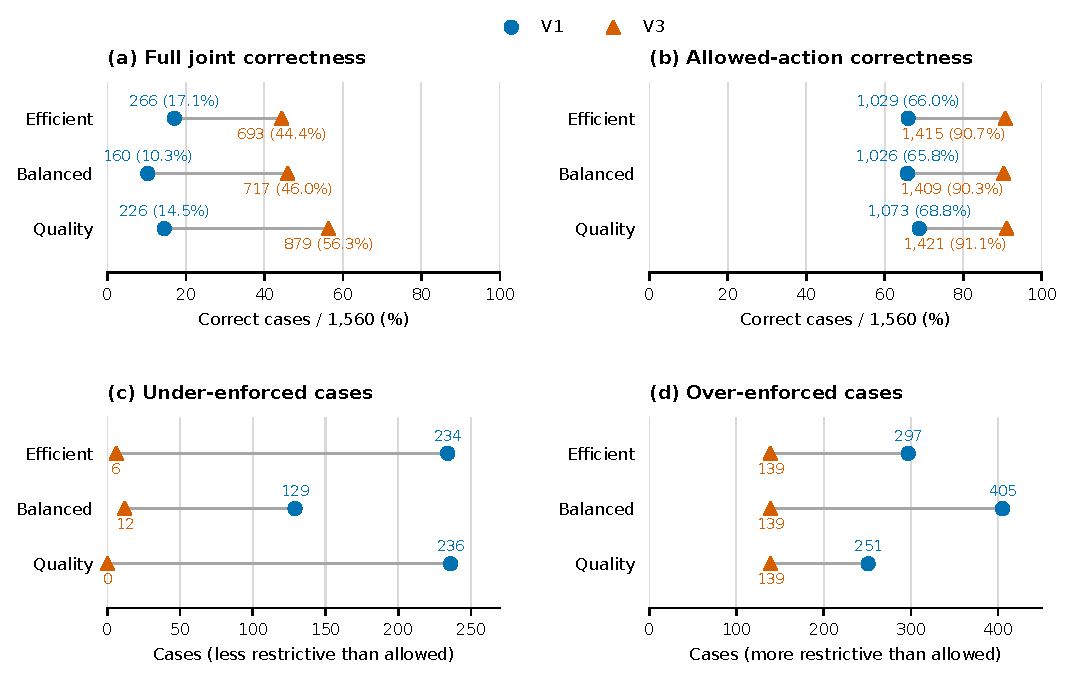
\includegraphics[width=\textwidth]{results-pipeline-v1-v3.pdf}
\caption{Detailed product comparison on 1,560 reused provisional cases. V1 denotes historical and V3 updated packages; joint means label-and-action joint agreement. Under/over-enforced panels count cases on different scales, not ordinal distance; native package differences prevent causal attribution.}
\label{fig:pipeline_v1_v3}
\end{figure*}
\begin{figure*}[t]
\centering
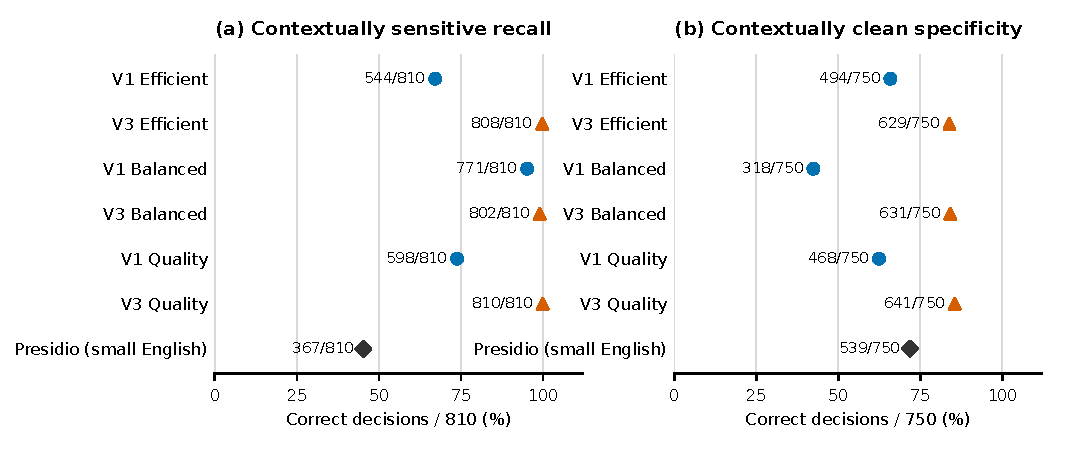
\includegraphics[width=\textwidth]{results-pipeline-presidio-reference.pdf}
\caption{Same-case binary reference: recall among 810 provisional sensitive and specificity among 750 clean cases. The diamond is small-English Presidio at threshold 0.5. PriVoke-authored reused data and entity/contextual task mismatch preclude an independent privacy ranking.}
\label{fig:pipeline_presidio_reference}
\end{figure*}

\section{Related-System Interaction Detail}
\label{app:interaction}
Table~\ref{tab:related_functions} distinguishes the reviewed systems by what happens to a prompt, warning and response. Table~\ref{tab:related_results} preserves selected reported outcomes with their own populations and metric boundaries. Together they inform design choices without supplying a matched effectiveness comparison: restoring a hidden entity, cancelling a request and matching a policy label are different outcomes.
\begin{table}[H]
\centering
\caption{Interaction functions reported in the reviewed versions. “Not described” is limited to the cited version and review scope.}
\label{tab:related_functions}
\small
\begingroup
\setlength{\tabcolsep}{3pt}
\begin{tabular}{>{\raggedright\arraybackslash}p{.18\columnwidth}>{\raggedright\arraybackslash}p{.39\columnwidth}>{\raggedright\arraybackslash}p{.35\columnwidth}}
\toprule
System & Prompt and response handling & Warning, acknowledgement and request effect \\
\midrule
Casper v1~\cite{CasperPreprintV12024} & Replaces identifiers and restores them in responses. & Topic warning has an acknowledgement control; user can inspect or restore. \\
HaS v1~\cite{HaS2024} & Hides entities and locally restores response entities. & Browser warning acknowledgement and request blocking not described. \\
ProSan v1~\cite{ProSan2024} & Selectively rewrites prompt words; evaluates downstream utility proxies. & Browser warning acknowledgement and request blocking not described. \\
PriVoke & ALLOW/WARN forward original body; returned masked spans are not substituted. & WARN notice is not awaited; BLOCK cancels supported requests. \\
\bottomrule
\end{tabular}
\endgroup
\end{table}



\begin{table}[t]
\centering
\caption{External reported outcomes on different tasks; no cross-study ranking or local reproduction.}
\label{tab:related_results}
\small
\begin{tabular}{>{\raggedright\arraybackslash}p{.23\columnwidth}>{\raggedright\arraybackslash}p{.29\columnwidth}>{\raggedright\arraybackslash}p{.33\columnwidth}}
\toprule
Work & Selected reported outcome & Population / boundary \\
\midrule
Casper v1 (2024)~\cite{CasperPreprintV12024} & NER recall 98.5\%, specificity 86.7\% & Two GPT-4-Turbo-generated 2,000-prompt workloads; NER support is 1,000 positive / 1,000 negative. \\
Casper 2025~\cite{CasperAbstract2026} & PII accuracy 92.6\% & Published abstract: 4,500 synthetic/2,000 real-world prompts; metric support unavailable. Separate from v1. \\
HaS v1 (2023)~\cite{HaS2024} & Black-box label-based protection 0.4070 & 19,703-example train/test corpus, 80/20; 1.7B black-box attacker; one minus whole-text recovery similarity, not entity protection; exact test support unspecified. \\
ProSan v1 (2024)~\cite{ProSan2024} & Local-star privacy hiding rate 99.8\% & MedQA, SAMSum and CodeAlpaca, 1,000 test prompts each; item-replacement proxy, exact item count unspecified. \\
PromptShield 2025~\cite{PromptShieldAbstract2026} & Policy accuracy 72.92\% & Independent 435-prompt test; full model/class supports unavailable. \\
\bottomrule
\end{tabular}
\end{table}
The reviewed ProSan v1 also requires WordNet similarity below 0.9 for occupation, race and orientation replacements. This constrains the replacement values, but the resulting item rate remains distinct from a prompt-level privacy measure.

\section{Selected Training Lineage}
\label{app:lineage}
PH3 began the selected lineage by fitting affine privacy heads over frozen pretrained encoders/poolers. It used 6,240 TRAIN and 1,560 validation rows, AdamW rate 0.001 and validation-selected checkpoints. EN3 then jointly fitted each selected parent's encoder, pooler and heads on the same data. AU3, repository protocol \texttt{ba7f3990}, added 3,120 audience rows alongside unchanged 6,240-row PH3 rehearsal and used a new 1,560-row validation set.

EN3/AU3 training used CPU-four-thread float32 execution, encoder/pooler rate $2\times10^{-5}$, head rate $10^{-4}$, weight decay 0.01, dropout 0.1 and microbatch 16/effective batch 64. The final incomplete batch contributed loss with its actual denominator. AU3 used 147 warmup updates and allowed 5--30 epochs, stopping after five validation epochs without strict $10^{-4}$ loss improvement. Checkpoint selection depended only on validation; sealed comparisons selected neither a model nor a threshold or recipe.

Table~\ref{tab:lineage} reports the ancestry actually selected for PIPE3. AU3 completed 16/11/9 epochs but selected checkpoints at 11/6/4; discarded optimization is excluded from the ancestry count. Cumulative selected encoder/pooler epochs were 30/20/8 and head epochs 42/27/12. V1 encoders had zero optimizer-trained epochs, while bootstrap heads had 220/360/520. These counts describe task-training history only and neither include nor equate to unknown upstream linguistic pretraining.

\begin{table}[H]
\centering
\caption{Selected V3 ancestry. Parameters are V1/V3 millions; PH3 is head-only, EN3/AU3 jointly train encoder, pooler and heads.}
\label{tab:lineage}
\small
\begin{tabular}{lrrrr}
\toprule
Tier & Parameters(M) & PH3 & EN3 & AU3 \\
\midrule
Efficient &.019/4.785 &12 &19 &11 \\
Balanced &.037/9.596 &7 &14 &6 \\
Quality &.054/17.494 &4 &4 &4 \\
\bottomrule
\end{tabular}
\end{table}



\section{Installed-Browser Cost Protocol}
\label{app:browser_protocol}
The cost protocol allocated two fresh profiles to each transport/action cell, for twelve profiles in total. Each profile contributed one first decision, five warmups and thirty measured regex/NER [2,3] requests; regex BLOCK could legitimately skip NER. The thirty-three correctness/fault probes ran outside these resource windows. The container exposed 24 processors with no CPU or memory quotas and reused resident fixture, driver and Go infrastructure.

Each observation window began before browser launch and ended after request/readiness checks, before profile teardown. Infrastructure startup before the window contributed no measured CPU, while resident services and cache remained in the memory total. The startup boundary consequently describes the instrumented fresh-profile/native path rather than an otherwise empty machine. No unprotected baseline was included.

Page-observed decision latency spanned the analysis-request and analysis-result messages, excluding the receiver response. Pooled nearest-rank percentiles described two session clusters; p99 was the observed maximum, not an independently estimated tail interval. The collector requested 100-ms sampling but retained each positive actual gap. CPU-counter differences spanned first-to-last observations, and the final read began after the last request, boundary checks and stop request.

Cgroup CPU totals included descendants, while sampled charged memory included cache and kernel charges and was not RSS/PSS~\cite{LinuxCgroupV2Interfaces2026}. Chromium, runtime, Go services, fixture, driver and observer all contributed; observer CPU was not subtracted. Boundary checks verified known browser/supervisor/detector identities, parent links, running status and listeners. This established boundary observations without continuous process attribution, native ancestry or incremental firewall overhead. The protocol required cleanup, and its nine earlier failed captures remain separate and unpooled.



\section{Descriptive Product Cost}
\label{app:product_cost}
The product measurements in Table~\ref{tab:cost} pair lower V3 first-pass host RPC medians with larger process peak RSS. V3 ran first, and the packages differed in NumPy/Torch backends, warming and cascade shortcuts. The observed timings therefore do not establish a controlled model speedup. Historical service timers and Linux lifetime-memory measurements cover different scopes and cannot supply the missing attribution or a model-only cost estimate.

\begin{table}[H]
\centering
\caption{PIPE3 descriptive cost: V1/V3 host RPC median(p95) ms and server-process peak RSS MiB. Excludes browser operation.}
\label{tab:cost}
\small
\begin{tabular}{lll}
\toprule
Tier & Median(p95), V1/V3 & RSS, V1/V3 \\
\midrule
Efficient &55.20(70.08)/43.71(50.12) &389.4/466.8 \\
Balanced &65.87(85.65)/42.73(47.82) &389.8/506.4 \\
Quality &59.58(90.08)/50.02(59.48) &391.8/523.4 \\
\bottomrule
\end{tabular}
\end{table}



\section{Installed-Browser Cost Outcomes}
\label{app:browser_cost}
Twelve completed fresh-profile windows produced the 360 decisions in Table~\ref{tab:browser_cost}. All 240 ALLOW/WARN measurements executed regex and NER; all 120 BLOCK measurements executed regex and legitimately skipped NER. Browser-context creation had nearest-rank p50 1.30 s, range 1.28--9.70; configuration/readiness transition had p50 4.37 s, range 4.21--12.21; the first post-readiness decision had p50 66.4 ms, range 53.6--75.2. These separately instrumented intervals do not combine into a model-only or cold-machine startup measurement.

\begin{table}[H]
\centering
\caption{Instrumented page-observed decision latency in ms for three fixed synthetic cases, requested regex/NER [2,3]. Each cell has sixty measurements in two fresh profiles; p99 is the observed maximum. Excludes receiver response and semantic-layer cost.}
\label{tab:browser_cost}
\small
\begin{tabular}{llrrr}
\toprule
Transport & Action & p50 & p95 & p99 \\
\midrule
fetch &ALLOW &35.0 &62.5 &73.6 \\
fetch &WARN &31.9 &36.1 &59.4 \\
fetch &BLOCK &27.9 &31.6 &33.2 \\
XHR &ALLOW &30.8 &35.8 &57.7 \\
XHR &WARN &31.3 &34.6 &59.2 \\
XHR &BLOCK &28.5 &32.2 &34.1 \\
\bottomrule
\end{tabular}
\end{table}

Summed window spans totalled 126.40 s, with aggregate container CPU of 193.29 s including 0.69 s of sampled observer CPU. Maximum sampled cgroup charged memory reached 1,267.91 MiB, including resident services and cache. The 1,236 samples produced 1,224 within-window gaps: median/p95/maximum 101.21/102.38/622.84 ms, with one gap above 500 ms. CPU accumulates concurrent work rather than wall time, and charged memory differs from process RSS/PSS; sampling gaps also leave possible spikes unseen. Final-read coverage and process/listener cleanup passed, followed by natural container exit with status zero. This establishes a completed capture, while its whole-container boundary still prevents isolating client overhead or comparing speed with Table~\ref{tab:cost}.



\section{Telemetry and Local Reconstruction Details}
\label{app:telemetry_reconstruction}
The finite audit enumerated exact rational kernels for the five implemented domains, $K=3,4,11,2,6$, on a fingerprinted Windows CPython 3.11.9 build. Outward 100-digit logarithm enclosures showed maximum event loss exceeding nominal $\varepsilon=0.5,1,2$ by approximately $1.294\times10^{-15}$, $1.503\times10^{-15}$ and $1.226\times10^{-15}$, respectively. Although small, these excesses invalidate an exact nominal bound for the audited settings. Under the same entropy assumptions, eight default reservations compose to approximately $8+1.202\times10^{-14}$. The result remains host- and setting-specific, without certifying other configurations or deployed builds.

Utility was assessed in 180 fixed-truth simulation cells, each repeated 10,000 times. For balanced integer category counts, $K=11$, event $\varepsilon=1$ and $n=80/8000$ reports, the first-category truth was $7/727$. Clipped bias reached $+22.84/+237.50$ and RMSE $42.32/1028.47$ counts. Clipping occurred in $85.62/28.32\%$ of trials; separately estimated marginals failed to sum to $n$ in $99.99/99.78\%$. The larger contributor count pools installation-days, with each still subject to the default eight-reservation cap.

The reported errors condition on realized contributor counts and omit population sampling. Simulation also approximates exact finite-kernel probabilities in binary64. Numerical moment and collector checks support consistency of that implemented estimation procedure, while leaving the acceptable error for a deployment use case unspecified.

Isolated ledger checks admitted eight reservations, denied the ninth, retained the cap after process reopen and reset it on the next UTC day. Rollback or corruption failed closed; forty concurrent epsilon-0.5 requests admitted sixteen reservations. Build, queue and delivery failures consumed their reservations as well. Reversing a constructed 32-event sequence containing 25\% BLOCK changed BLOCK representation among the first-eight contributors from 100\% to 0\%. This establishes selection sensitivity before randomization, without measuring real deployment monitoring accuracy.
\subsection{Local Source/Model Reconstruction}
A separately sealed local capsule contained 195 pins: the 158 runtime files from the later FN14 freeze, additional helpers, six frozen V1/AU3 model bundles and prior invented probe receipts. Its inventory differs from the historical 154-file clean-checkout comparison. Six fresh host servers loaded isolated source copies and replayed four invented sole-semantic requests per package. All 24 classifications/actions and four package identity fields matched without errors; independent post-run checks verified pins, import origins and process cessation. This establishes bounded reconstruction in the maintained Python environment, without establishing public Git-only installation, fresh-dependency reproduction, accuracy or a protected-final rerun.


\subsection{Implemented Finite Kernel}
To calculate finite privacy loss, the audit follows the sampler's threshold comparison rather than assuming ideal randomized-response probabilities. Let $\widetilde p_i$ be the binary64 truth threshold. The audited CPython implementation draws a fresh uniform 53-bit integer $J$ and selects truth when $J/2^{53}<\widetilde p_i$, giving
\begin{equation}
\begin{aligned}
P_i&=\frac{\lceil2^{53}\widetilde p_i\rceil}{2^{53}},\quad Q_i=\frac{1-P_i}{K_i-1},\\
\varepsilon_{\rm finite}&=\sum_i\log\max\{P_i/Q_i,Q_i/P_i\}.
\end{aligned}
\end{equation}
Alternative selection uses rejection sampling. The calculation assumes independent uniform OS bits and the fingerprinted host's arithmetic; it therefore supplies no independent certification of deployment entropy or other builds.

\bibliographystyle{ieeetr}
\bibliography{ref,research/paper-completion-sources-20261014,manuscript-completion-sources-20261014,research/literature-baseline-sources-20261015}
\end{document}
